\documentclass{article}
\usepackage{times}
\usepackage{graphicx}
\usepackage{subfigure} 
\usepackage{hyperref}
\usepackage{amsmath}
\usepackage{amssymb}
\begin{document}
	%Ghassen
	\section{LM ARIMA}

	%Tom
	\section{Grid Search for the Most Promising Parameters}
	
        See http://tiny.cc/grid_search_results


	%Vlad
	\section{Kelly trading strategy}
	
The primary means through which our analysis is replicable, falsifiable, and quantitatively assessable is by assessing investment performance. Raw accuracy of prediction does not present a fair evaluation of our algorithm, since we need to consider inherent difficulties with predicting the market. In other words, if we make a significant amount of money (e.g. compare the mean returns to S\&P alpha), then there is some inefficiency in the market that our algorithm correctly enables us to take advantage of.

We will use strong simplifying assumptions: we can trade stock at any volume at the EOD price instantaneously without affecting the market. To some extent these assumptions can hold assuming we create a portfolio of commodities, which artificially lowers market presence in individual ones.

That said, we need to convert our model into an actual strategy. Consider the random variable for the EOD price of a commodity $p_i$ for day $i$. Our LM and ARIMA Models provide for $X = \log\frac{p_{i+1}-p_i}{p_i}$ and $X'=X|p_{<i},\text{news}$ an estimate $\mu=\mathbb{E}(X')$ and $\sigma^2=\mathbb{V}(X')$.

The Kelly Criterion (in the continuous case) gives the optimal betting proportion (given an investment, you should only bet a part of it if you're unsure and leverage it if you aren't). This doesn't make any stronger assumptions about the returns (which should be normal about our prediction) than the models do. Then, each day, we need to buy or short sell $\text{sgn }\mu\cdot\frac{\left|\mu\right|-r}{\sigma^2}$ proportion of our investment, where we sell or buy back all our holdings the next day. We purchase leverage at the risk-free rate $r$, so we only invest when we can earn over that much.

Source: http://wwwf.imperial.ac.uk/~mdavis/docs/DavisLleoKellyChapter.pdf

Here's an example run. The purple line is a trading strategy with $\mu\sim\text{Unif}(-5,5)$ and the tan line has $\mu\sim\text{Unif}(-1,1)$. Both have $\sigma^2\sim\text{Unif}(0.25,10)$. The following has $r=0$:

\begin{center}
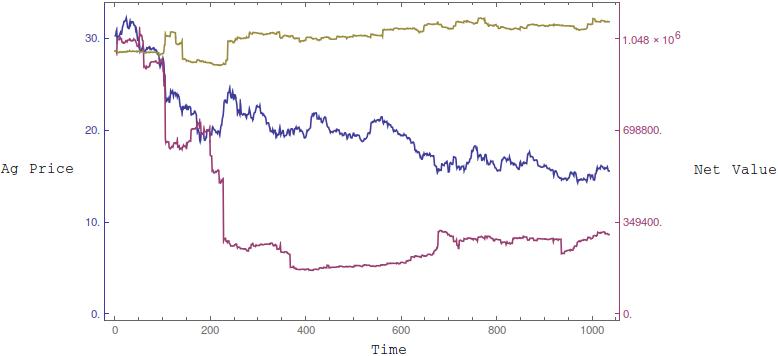
\includegraphics[scale=0.5]{../KellyRun-Random.png}
\end{center}

Notice when we're really confident we tend to leverage {\em a lot}. We might want to have a minimum uncertainty bound, maybe based on stock volatility.

	%Daway
		\section{Clustering}
	
	We attempted using a Dirichlet Process GMM because we have relatively information for deciding how many news clusters there should be. Unfortunately, implementations we attempted to use were intractable given the memory and computing constraints of the ionic cluster. Thus we had to revert back to a $K$-means clustering model.

	We train these models on a set of randomly sampled events for a given date range, for example, the date range of 01-01-2006 to 12-31-2013. Currently we sample 600,000 events across 150 randomly chosen files in this range, weighting the number of events from each day according to the total number of events in that day. Since trading strategies occur day by day, we can train this clustering offline and then make an "online" prediction for which cluster the next day's news data will belong in.

	Since we must do a parameter search across various values for $K$, we do a manual eyeball test to see if clusters make sense. With so many events, values for $K=1000$ or greater seem reasonable. We will present qualitative assessments for some clusters in the $K=1000$ model. It will be easiest to describe the raw news events with the url associated with them.

	Sometimes we can see logical reasons for clusters even if they might not be the most natural or related clusters. For example, cluster 2 has many news related to police:
	\begin{enumerate}
	\item http://www.stgeorgeutah.com/news/archive/2014/12/31/cmm-department-honors-retiring-fire-chief-with-36-booms-and-a-bell/
	\item https://news.vice.com/article/georgia-police-chief-claims-he-accidentally-shot-wife-on-new-years-day
	\item
	http://news.gnom.es/news/nyc-to-ring-in-new-year-with-heightened-security-in-times-square
	\end{enumerate}

	Many times, clusters seem to have many mini-clusters in them. We see this in cluster 345, which has a lot of news related to Israel/Palestine, but also a lot of news related to generate gun violence.
	\begin{enumerate}
	\item http://www.israelherald.com/index.php/sid/228975387
	\item http://www.breakingisraelnews.com/26803/indiana-governor-mike-pence-pledges-support-from-heartland-of-israel-jerusalem/
	\item http://www.thedenverchannel.com/newsy/how-palestinian-leaders-latest-move-could-backfire
	\item http://www.erietvnews.com/story/27744858/mahmoud-abbas-fast-facts
	\item http://www.bostonglobe.com/metro/2015/01/01/brandeis-student-stands-comments-after-slayings-new-york-police-officers/oLpI7MiV42hk3ymM05QzLN/story.html
	\item http://www.toledoblade.com/State/2015/01/01/Cleveland-seeks-outside-probe-of-boy-s-shooting.html
	\end{enumerate}

	There were many clusters that had good topic clustering, such as general politics clusters, which would contain news about gubernatorial elections, general actions by President Obama, and some foreign policy news. But overall, these clusters were disappointing since they didn't leverage geographic location to separate clusters that way which we would have suspected. 

	One of the best clusters found had to do with general crime and legal issues, though again, geographic information does not seem to have affected clustering much. We also note that the magnitude or importance of these events does not seem to match up.
	\begin{enumerate}
	\item http://blogs.reuters.com/faithworld/2015/01/01/new-zealand-bar-manager-pleads-not-guilty-to-insulting-buddhism-in-myanmar/
	\item http://www.hstoday.us/blogs/the-kimery-report/blog/cia-might-have-avoided-post-911-torture-charges-had-it-remembered-beirut-1983/eb540ef9ce52b4a80f490369e743e4fb.html
	\item http://www.military.com/daily-news/2015/01/01/us-sends-5-detainees-to-kazakhstan-a-day-late.html?comp=700001075741rank=4
	\item http://aninews.in/newsdetail4/story197991/lakhvi-sent-to-14-days-judicial-custody-in-kidnapping-case.html
	\item http://www.sasklifestyles.com/news/police-say-mother-of-missing-14-month-old-maryland-boy-left-him-on-stranger-s-porch-in-ohio-1.1700200
	\end{enumerate}

	Overall, most clusters had some sort of relating factor for its news events. But the main problems we can identify are the existence of multiple mini clusters and the division of true clusters across many clusters. The second point might be less worrisome, since the $K$-means algorithm may have split these "true clusters" because of magnitude and importance features which are harder to eyeball than assigning topics.
\begin{enumerate}
\item http://blogs.reuters.com/faithworld/2015/01/01/new-zealand-bar-manager-pleads-not-guilty-to-insulting-buddhism-in-myanmar/
\item http://www.hstoday.us/blogs/the-kimery-report/blog/cia-might-have-avoided-post-911-torture-charges-had-it-remembered-beirut-1983/eb540ef9ce52b4a80f490369e743e4fb.html
\item http://www.military.com/daily-news/2015/01/01/us-sends-5-detainees-to-kazakhstan-a-day-late.html?comp=700001075741rank=4
\item http://aninews.in/newsdetail4/story197991/lakhvi-sent-to-14-days-judicial-custody-in-kidnapping-case.html
\item http://www.sasklifestyles.com/news/police-say-mother-of-missing-14-month-old-maryland-boy-left-him-on-stranger-s-porch-in-ohio-1.1700200
\end{enumerate}

Overall, most clusters had some sort of relating factor for its news events. But the main problems we can identify are the existance of multiple mini clusters and the division of true clusters across many clusters. The second point might be less worrisome, since the $K$-means algorithm may have split these "true clusters" because of magnitude and importance features which are harder to eyeball than assigning topics. 

\end{document}
